\chapter{Searching Algorithms}

The search tree data structure supports many dynamic-set operations, including
SEARCH, MINIMUM, MAXIMUM, PREDECESSOR, SUCCESSOR, INSERT, and
DELETE. Thus, we can use a search tree both as a dictionary and as a priority
queue.
Basic operations on a binary search tree take time proportional to the height of
the tree. For a complete binary tree with n nodes, such operations run in $\Theta(\log n)$
worst-case time. If the tree is a linear chain of n nodes, however, the same oper-
ations take $\Theta(n)$ worst-case time. We shall see that the expected height of a randomly
built binary search tree is only $\Theta(\log n)$, so that the \textbf{expected} time for these 
operations is $\Theta(\log n)$.


\section{Binary Search Trees}

We can represent a binary tree by a linked data structure in which each node is an object.
In addition to a \textbf{key} and \textbf{satellite} data, each node contains attributes \textbf{left}, \textbf{right}, and \textbf{p} that
point to the nodes corresponding to its left child, its right child, and its parent, respectively.

\begin{itemize}
    \item \textbf{Input}: a SORTED sequence of n keys 
    \item \textbf{Output}: a position i in the sequence where the key is located
\end{itemize}

\begin{figure}[H]
    \centering
    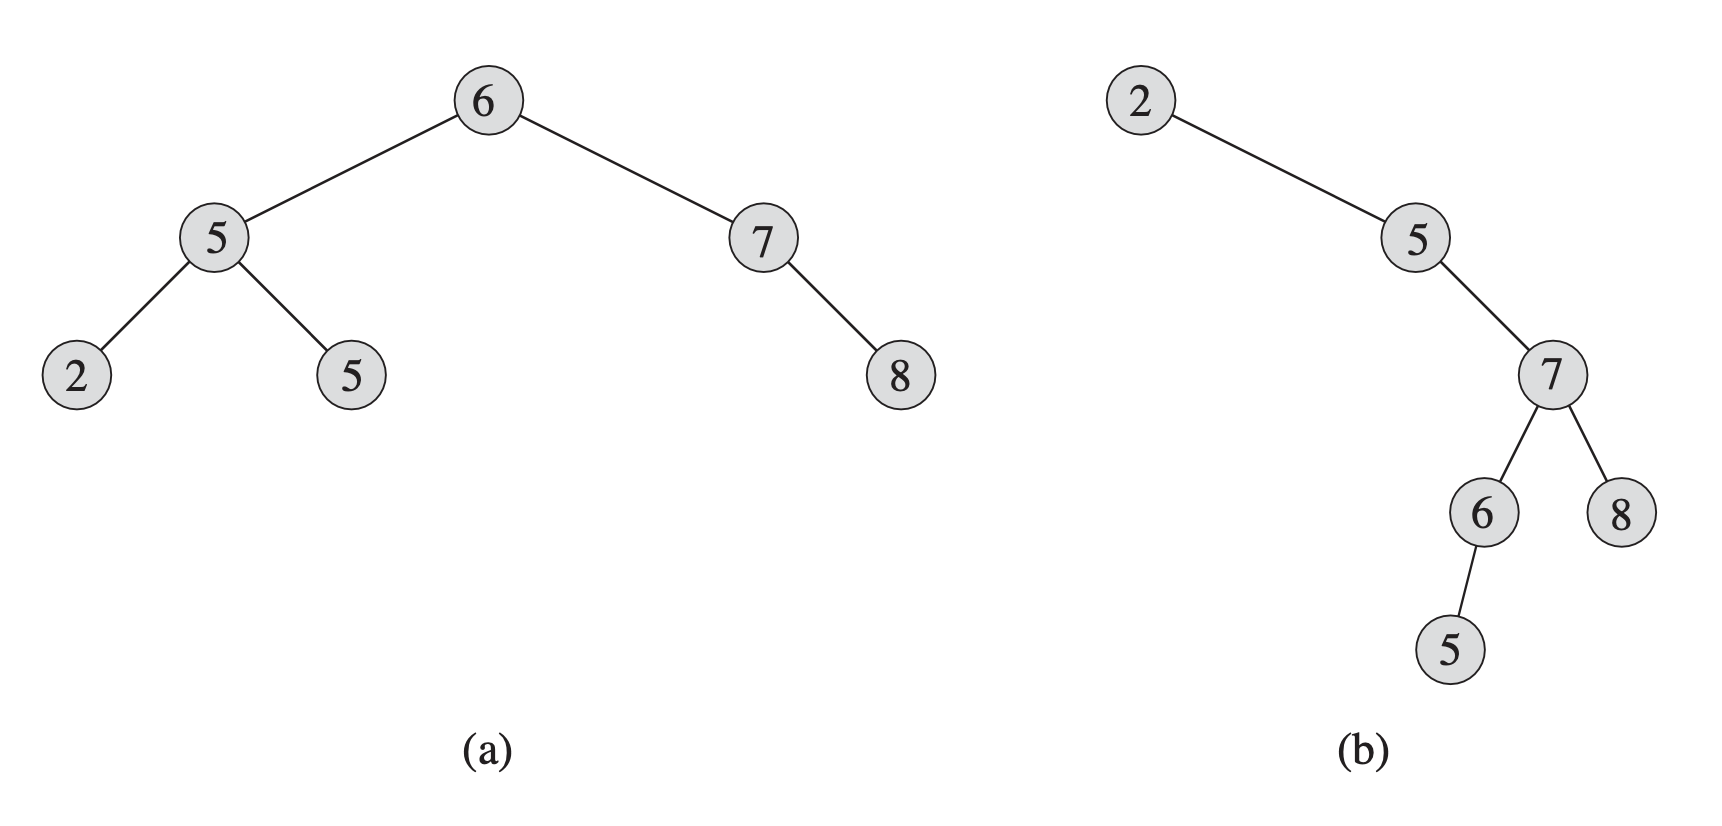
\includegraphics[width=0.7\textwidth]{assets/binary_tree.png}
    \caption{Binary Search Tree}
\end{figure}

The keys in a binary search tree are always stored in such a way as to satisfy the
\textbf{binary-search-tree property}:

\begin{definitionblock}[Binary Search Tree Property]
Let x be a node in a binary search tree. If y is a node in the left subtree of x, then $y.key \leq x.key$. If y is a node in the right subtree of x, then $y.key \geq x.key$.
\end{definitionblock}

The binary-search-tree property allows us to print out all the keys in a binary
search tree in sorted order by a simple recursive algorithm, called an \textbf{inorder tree
walk}. This algorithm is so named because it prints the key of the root of a subtree
between printing the values in its left subtree and printing those in its right subtree.
(Similarly, a \textbf{preorder tree walk} prints the root before the values in either subtree,
and a \textbf{postorder tree walk} prints the root after the values in its subtrees.)

\begin{algorithm}[H]
    \caption{Inorder Tree Walk}
    \begin{algorithmic}[1]
        \If{x $\neq$ NIL}
            \State INORDER-TREE-WALK(x.left)
            \State print x.key
            \State INORDER-TREE-WALK(x.right)
        \EndIf
    \end{algorithmic}
\end{algorithm}

It takes $\theta(n)$ time to walk an n-node binary search tree, since after the initial call, the procedure calls itself recursively exactly twice for each node in the tree: once for its left child and once for its right child.

\newtheorem{binary search}{theorem}

\begin{theorem}
    The complexity of \small INORDER-TREE-WALK \normalsize on a $n$ nodes binary search tree is $\Theta(n)$.
\end{theorem}

\begin{proof}
    \begin{align*}
    T(n) &\leq T(k) + T(n-k-1) + d \\
    &= ((c + d)k + c) + ((c + d)(n - k - 1) + c) + d \\
    &= (c + d)n + c - (c + d) + c + d \\
    &= (c + d)n + c,
    \end{align*}
    Where c and d are constants that represent the time per call to INORDER-TREE-WALK and the time per print statement, respectively.  $k$ is the number of nodes in the left subtree of $x$, while $n - k - 1$ is the number of nodes in the right subtree of $x$. The base case occurs when $n = 0$, in which case the running time is constant. The recurrence is linear, and so the running time of INORDER-TREE-WALK is \small{$\Theta(n)$}.
\end{proof}

\subsection{Quering a Binary Search Tree}

We often need to search for a key stored in a binary search tree. Besides the SEARCH operation, binary search trees can support such queries as MINIMUM, MAXIMUM, SUCCESSOR, and PREDECESSOR. In this section, we shall examine these operations and show how to support each one in time $O(h)$ on any binary search tree of height $h$.

\vspace{-0.5em}

\subsubsection*{Searching}

\begin{definitionblock}[Searching]
    We use the following procedure to search for a node with a given key in a binary search tree. Given a pointer to the root of the tree and a key $k$, TREE-SEARCH returns a pointer to a node with key $k$ if one exists; otherwise, it returns NIL.
\end{definitionblock}

\begin{algorithm}[H]
    \caption{TREE-SEARCH(x, k)}
    \begin{algorithmic}[1]
        \While{x $\neq$ NIL \textbf{ and } k $\neq$ x.key}
            \If{k < x.key}
                \State x $\gets$ x.left
            \Else
                \State x $\gets$ x.right
            \EndIf
        \EndWhile
        \State \Return x
    \end{algorithmic}
\end{algorithm}

\subsubsection*{Minimum and Maximum}

We can always find an element in a binary search tree whose key is a minimum by
following left child pointers from the root until we encounter a NIL.

\begin{algorithm}[H]
    \caption{TREE-MINIMUM(x)}
    \begin{algorithmic}[1]
        \While{x.left $\neq$ NIL}
            \State x $\gets$ x.left
        \EndWhile
        \State \Return x
    \end{algorithmic}
\end{algorithm}

Same for the maximum:

\begin{algorithm}[H]
    \caption{TREE-MAXIMUM(x)}
    \begin{algorithmic}[1]
        \While{x.right $\neq$ NIL}
            \State x $\gets$ x.right
        \EndWhile
        \State \Return x
    \end{algorithmic}
\end{algorithm}

Both of these procedures run in $O(h)$ time on a tree of height $h$ since, as in TREE-SEARCH, the sequence of nodes encountered forms a simple path downward from the root.

\subsubsection*{Successor and Predecessor}

Given a node in a binary search tree, sometimes we need to find its successor in the sorted order determined by an inorder tree walk. If all keys are distinct, the
successor of a node x is the node with the smallest key greater than x:key. The structure of a binary search tree allows us to determine the successor of a node
without ever comparing keys. The following procedure returns the successor of a node x in a binary search tree if it exists, and NIL if x has the largest key in the tree:

\begin{algorithm}[H]
    \caption{TREE-SUCCESSOR(x)}
    \begin{algorithmic}[1]
        \If{x.right $\neq$ NIL}
            \State \Return TREE-MINIMUM(x.right)
        \EndIf
        \State y $\gets$ x.p
        \While{y $\neq$ NIL \textbf{ and } x = y.right}
            \State x $\gets$ y
            \State y $\gets$ y.p
        \EndWhile
        \State \Return y
    \end{algorithmic}
\end{algorithm}

\subsection{Insertion and Deletion}

The operations of insertion and deletion cause the dynamic set represented by a
binary search tree to change. The data structure must be modified to reflect this
change, but in such a way that the binary-search-tree property continues to hold.

\subsubsection*{Insertion}

The procedure takes a node z for which $z.key = v$,$ z.left = NIL$ and $z.right = NIL$. 
It modifies the tree T and some of the attributes of z in such a way that it inserts
z into the appropriate position in the tree.

\begin{algorithm}[H]
    \caption{TREE-INSERT(T, z)}
    \begin{algorithmic}[1]
        \State y $\gets$ NIL
        \State x $\gets$ T.root
        \While{x $\neq$ NIL}
            \State y $\gets$ x
            \If{z.key < x.key}
                \State x $\gets$ x.left
            \Else
                \State x $\gets$ x.right
            \EndIf
        \EndWhile
        \State z.p $\gets$ y
        \If{y = NIL}
            \State T.root $\gets$ z
        \ElsIf{z.key < y.key}
            \State y.left $\gets$ z
        \Else
            \State y.right $\gets$ z
        \EndIf
    \end{algorithmic}
\end{algorithm}

\begin{figure}[H]
    \centering
    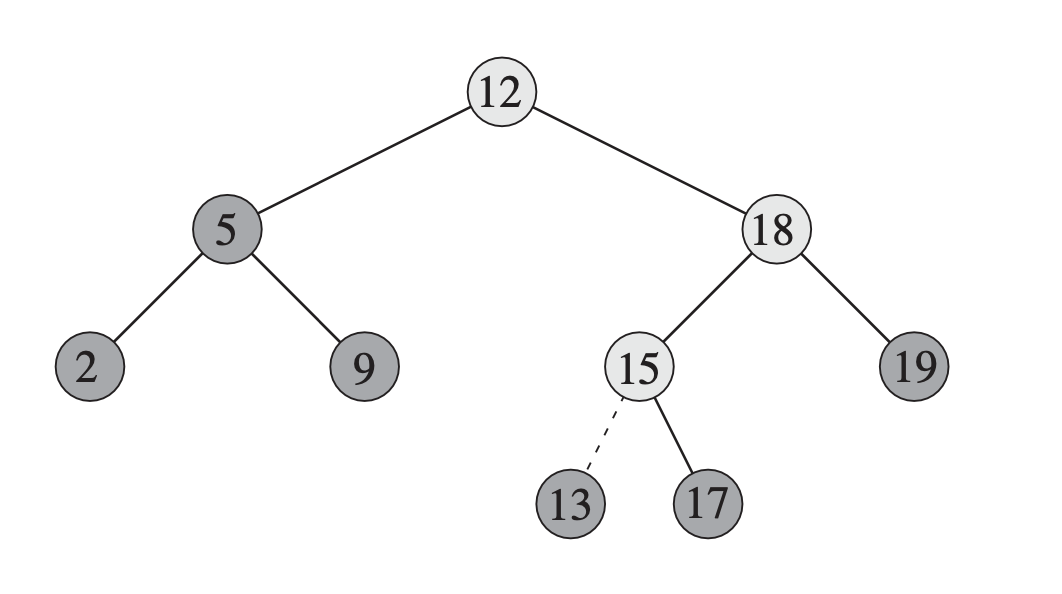
\includegraphics[width=0.5\textwidth]{assets/insertion_bt.png}
    \caption{Insertion in a Binary Search Tree}
\end{figure}

\subsubsection*{Deletion}

\begin{itemize}
    \item \textbf{Case 1}: If node z has no children, then we simply remove it by modifying its parent to replace z with NIL as its child.
    \item \textbf{Case 2}: If node z has just one child, then we elevate that child to take z’s position in the tree by modifying z’s parent to replace z by z’s child.
    \item \textbf{Case 3}: If node z has two children, then we find z’s successor y, which lies in z’s right subtree and has no left child. We want to splice y out of its current location and have it replace z in the tree.
\end{itemize}

\begin{algorithm}[H]
    \caption{TREE-DELETE(T, z)}
    \begin{algorithmic}[1]
        \If{z.left = NIL}
            \State TRANSPLANT(T, z, z.right)
        \ElsIf{z.right = NIL}
            \State TRANSPLANT(T, z, z.left)
        \Else
            \State y $\gets$ TREE-MINIMUM(z.right)
            \If{y.p $\neq$ z}
                \State TRANSPLANT(T, y, y.right)
                \State y.right $\gets$ z.right
                \State y.right.p $\gets$ y
            \EndIf
            \State TRANSPLANT(T, z, y)
            \State y.left $\gets$ z.left
            \State y.left.p $\gets$ y
        \EndIf
    \end{algorithmic}
\end{algorithm}

\begin{figure}[H]
    \centering
    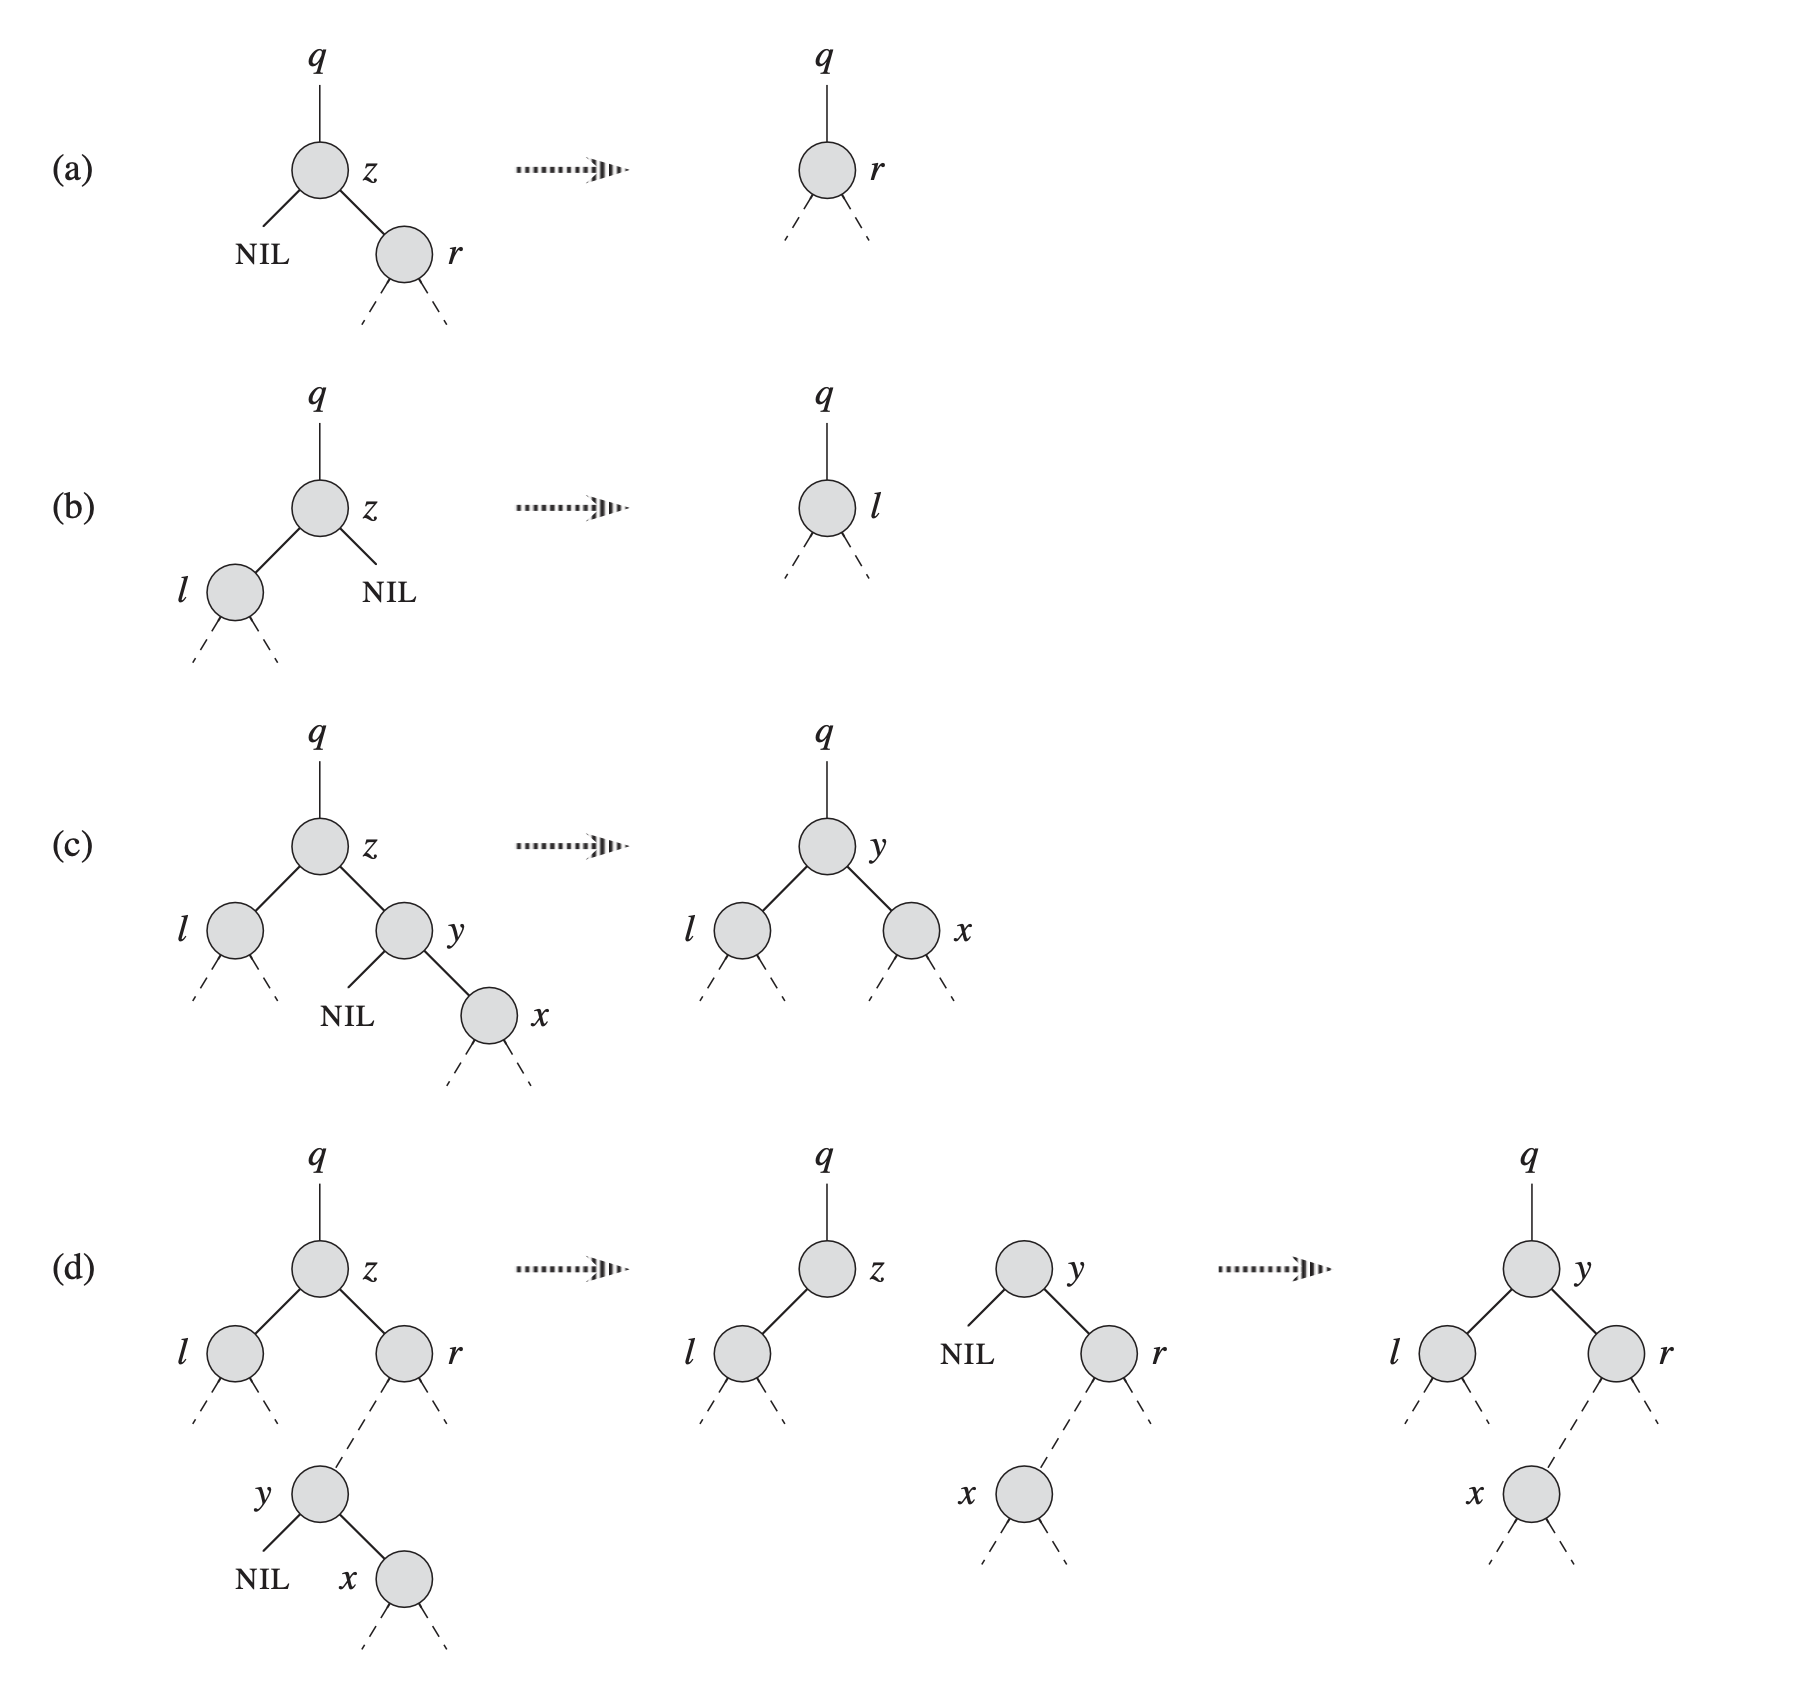
\includegraphics[width=0.8\textwidth]{assets/deletion_bt.png}
    \caption{Deletion in a Binary Search Tree.\\(a) Node $z$ has no left child.\\(b) Node $z$ has a left child but not a right child.\\(c) Node $z$ has two children.\\(d) Node z has two children, and its successor $y \neq r$ lies between the subtree rooted at $r$.}
\end{figure}

\begin{algorithm}[H]
    \caption{TRANSPLANT(T, u, v)}
    \begin{algorithmic}[1]
        \If{u.p = NIL}
            \State T.root $\gets$ v
        \ElsIf{u = u.p.left}
            \State u.p.left $\gets$ v
        \Else
            \State u.p.right $\gets$ v
        \EndIf
        \If{v $\neq$ NIL}
            \State v.p $\gets$ u.p
        \EndIf
    \end{algorithmic}
\end{algorithm}

\subsection*{Sorting}

\begin{algorithm}[H]
    \caption{BST-SORT(T)}
    \begin{algorithmic}[1]
        \State T $\gets \emptyset$
        \For{i = 1 \textbf{ to } n}
            \State T.root $\gets$ TREE-INSERT(T, i)
        \EndFor
        \State INORDER-TREE-WALK(T.root)
        \State \Comment{Time complexity: $\Theta(n \log n)$}
    \end{algorithmic}
\end{algorithm}

INORDER-TREE-WALK takes $\Theta(n)$ time, and we call it n times, so the total time is $\Theta(n \log n)$.

\section{Red-Black Trees}

It is a BST that enjoys the following properties:
\begin{itemize}
    \item Every node is colored, either \textbf{red} or \textbf{black}.
    \item The root is \textbf{black}.
    \item Every leaf (NIL) is \textbf{black}.
    \item If a \textbf{red} node has children, then the children are \textbf{black}.
    \item All paths from a node to its leaves have the same \textbf{black} height.
\end{itemize}

\begin{figure}[H]
    \centering 
    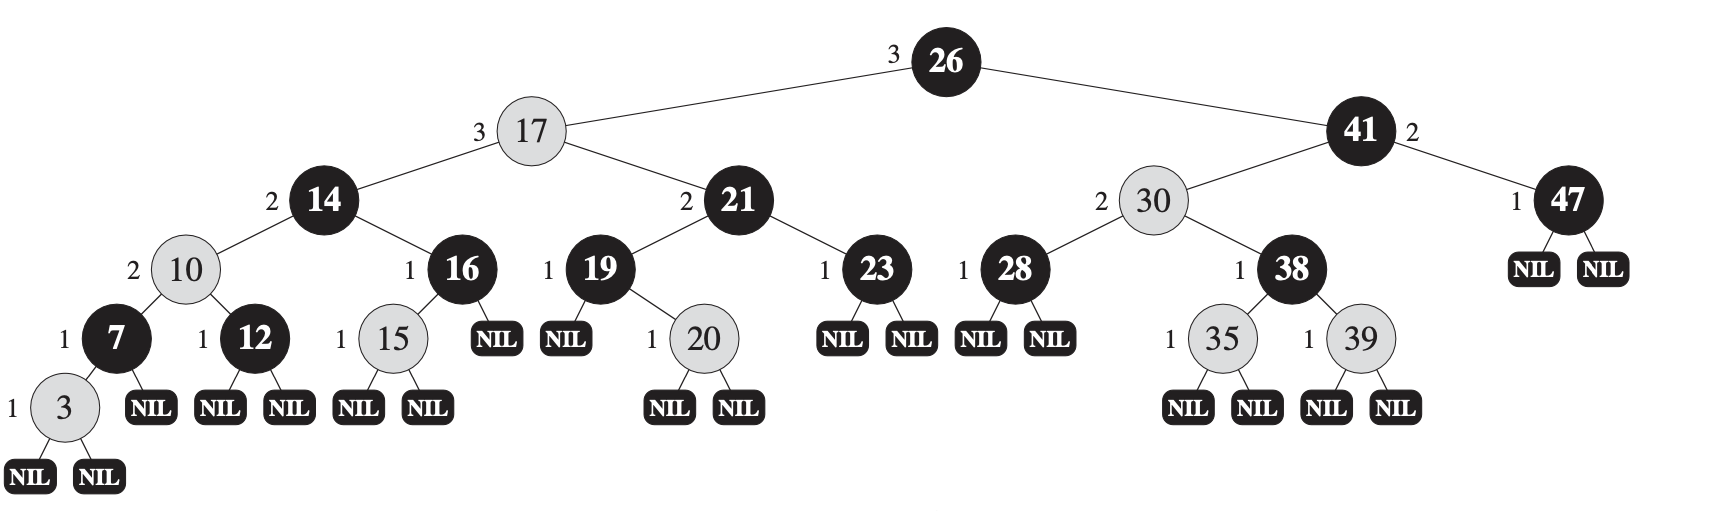
\includegraphics[width = \textwidth]{assets/RBT.png}
    \caption{Red-Black Tree}
\end{figure}

\newtheorem{RBT}{theorem}
\begin{theorem}
    Any Red-Black Tree with n keys has the height $h \leq 2\log(n+1)$
\end{theorem}
\begin{proof}
    We start by showing that the subtree rooted at any node $x$ contains at least $2^{\text{bh}(x)} - 1$ internal nodes. We prove this claim by induction on the height of $x$. If the height of $x$ is $0$, then $x$ must be a leaf ($T.\text{nil}$), and the subtree rooted at $x$ indeed contains at least 

    $$
    2^{\text{bh}(x)} - 1 = 2^0 - 1 = 0
    $$

    internal nodes.

    For the inductive step, consider a node $x$ that has positive height and is an internal node with two children. Each child has a black-height of either $\text{bh}(x)$ or $\text{bh}(x) - 1$, depending on whether its color is red or black, respectively. Since the height of a child of $x$ is less than the height of $x$ itself, we can apply the inductive hypothesis to conclude that each child has at least 

    $$
    2^{\text{bh}(x)-1} - 1
    $$ 

    internal nodes. Thus, the subtree rooted at $x$ contains at least 

    $$
    \left(2^{\text{bh}(x)-1} - 1\right) + \left(2^{\text{bh}(x)-1} - 1\right) + 1 = 2^{\text{bh}(x)} - 1
    $$ 

    internal nodes, which proves the claim.
\end{proof}

\vspace{-1em}

\subsection*{Rotations}

The operations TREE-INSERT and TREE-DELETE can violate the properties of a red-black tree. To restore these properties, we use two operations: LEFT-ROTATE and RIGHT-ROTATE.

\begin{algorithm}[H]
    \caption{LEFT-ROTATE(T,x)}
    \begin{algorithmic}[1]
        \State y $\gets$ x.right
        \State x.right $\gets$ y.left
        \If{y.left $\neq$ T.nil}
            \State y.left.p $\gets$ x
        \EndIf
        \State y.p $\gets$ x.p
        \If{x.p = T.nil}
            \State T.root $\gets$ y
        \ElsIf{x = x.p.left}
            \State x.p.left $\gets$ y
        \Else
            \State x.p.right $\gets$ y
        \EndIf
        \State y.left $\gets$ x
        \State x.p $\gets$ y
    \end{algorithmic}
\end{algorithm}

\vspace{-1em}

\begin{figure}[H]
    \centering
    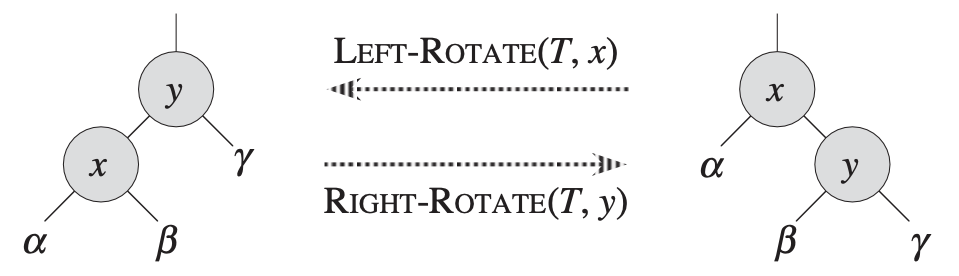
\includegraphics[width=0.5\textwidth]{assets/rotation_rbt.png}
    \caption{Left Rotation}
\end{figure}

\begin{figure}[H]
    \centering
    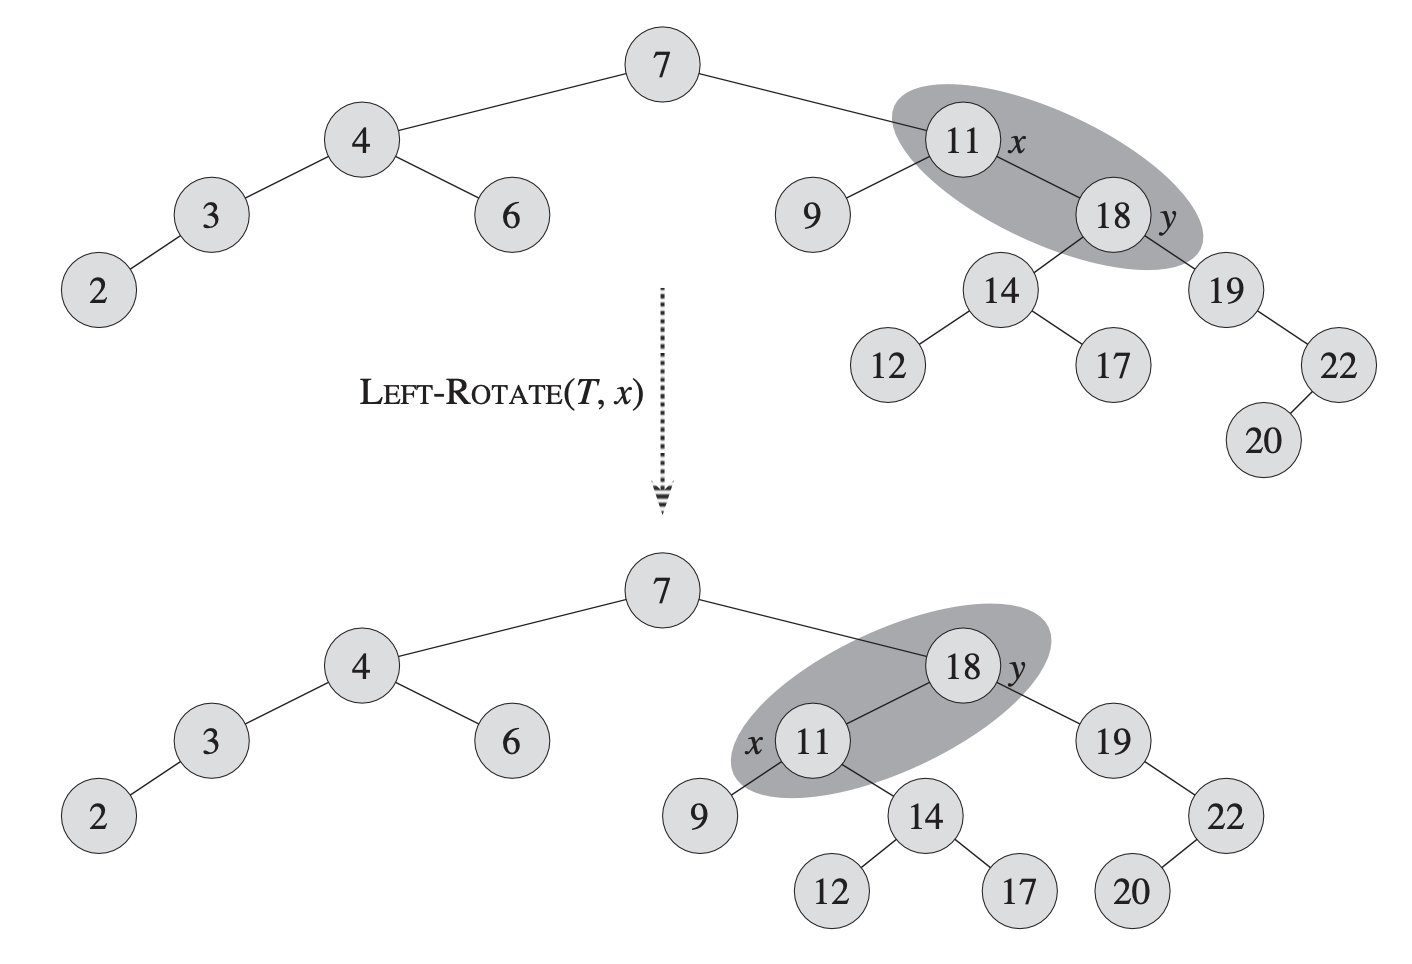
\includegraphics[width=0.7\textwidth]{assets/rotation_example_rbt.png}
    \caption{Example of rotation in a Red-Black Tree}
\end{figure}

\vspace{-1em}

\subsection*{Insertion}

We can insert a new node into a red-black tree by using the following procedure. The procedure takes as input the tree $T$ and a node $z$ to insert into $T$. It modifies the tree as necessary to maintain the red-black properties.

\begin{algorithm}[H]
    \caption{RB-INSERT(T,z)}
    \begin{algorithmic}[1]
        \State y $\gets$ T.nil
        \State x $\gets$ T.root
        \While{x $\neq$ T.nil}
            \State y $\gets$ x
            \If{z.key < x.key}
                \State x $\gets$ x.left
            \Else
                \State x $\gets$ x.right
            \EndIf
        \EndWhile
        \State z.p $\gets$ y
        \If{y = T.nil}
            \State T.root $\gets$ z
        \ElsIf{z.key < y.key}
            \State y.left $\gets$ z
        \Else
            \State y.right $\gets$ z
        \EndIf
        \State z.left $\gets$ T.nil
        \State z.right $\gets$ T.nil
        \State z.color $\gets$ RED
        \State RB-INSERT-FIXUP(T,z)
    \end{algorithmic}
    \hl
    Time complexity: $\Theta(\log n)$
\end{algorithm}

\subsubsection*{Why RB-INSERT-FIXUP is Necessary}

The \texttt{RB-INSERT-FIXUP} algorithm is necessary to maintain the properties of a red-black tree after the insertion of a new node. When a new node is inserted, it is initially colored red. This can potentially violate the red-black tree properties, specifically:

\begin{itemize}
    \item Property 2: The root must be black.
    \item Property 4: Both children of every red node must be black (no two red nodes can be adjacent).
    \item Property 5: Every path from a node to its descendant NIL nodes must have the same number of black nodes.
\end{itemize}

The \texttt{RB-INSERT-FIXUP} algorithm corrects any violations of these properties by performing a series of color changes and rotations. This ensures that the tree remains balanced, with a height of at most $2\log(n+1)$, which guarantees that the basic dynamic set operations (such as search, insert, and delete) can be performed in $O(\log n)$ time.

\begin{minipage}[H]{0.55\textwidth}
    \begin{algorithm}[H]
        \caption{RB-INSERT-FIXUP(T,z)}
        \begin{algorithmic}[1]
            \While{z.p.color = RED}
                \If{z.p = z.p.p.left}
                    \State y $\gets$ z.p.p.right
                    \If{y.color = RED}
                        \State z.p.color $\gets$ BLACK
                        \State y.color $\gets$ BLACK
                        \State z.p.p.color $\gets$ RED
                        \State z $\gets$ z.p.p
                    \Else
                        \If{z = z.p.right}
                            \State z $\gets$ z.p
                            \State LEFT-ROTATE(T,z)
                        \EndIf
                        \State z.p.color $\gets$ BLACK
                        \State z.p.p.color $\gets$ RED
                        \State RIGHT-ROTATE(T,z.p.p)
                    \EndIf
                \Else
                    \State \# Mirror case: perform same operations
                    \State \# with left/right reversed
                \EndIf
            \EndWhile
            \State T.root.color $\gets$ BLACK
        \end{algorithmic}
    \end{algorithm}
\end{minipage}%
\begin{minipage}[H]{0.45\textwidth}
    \centering
    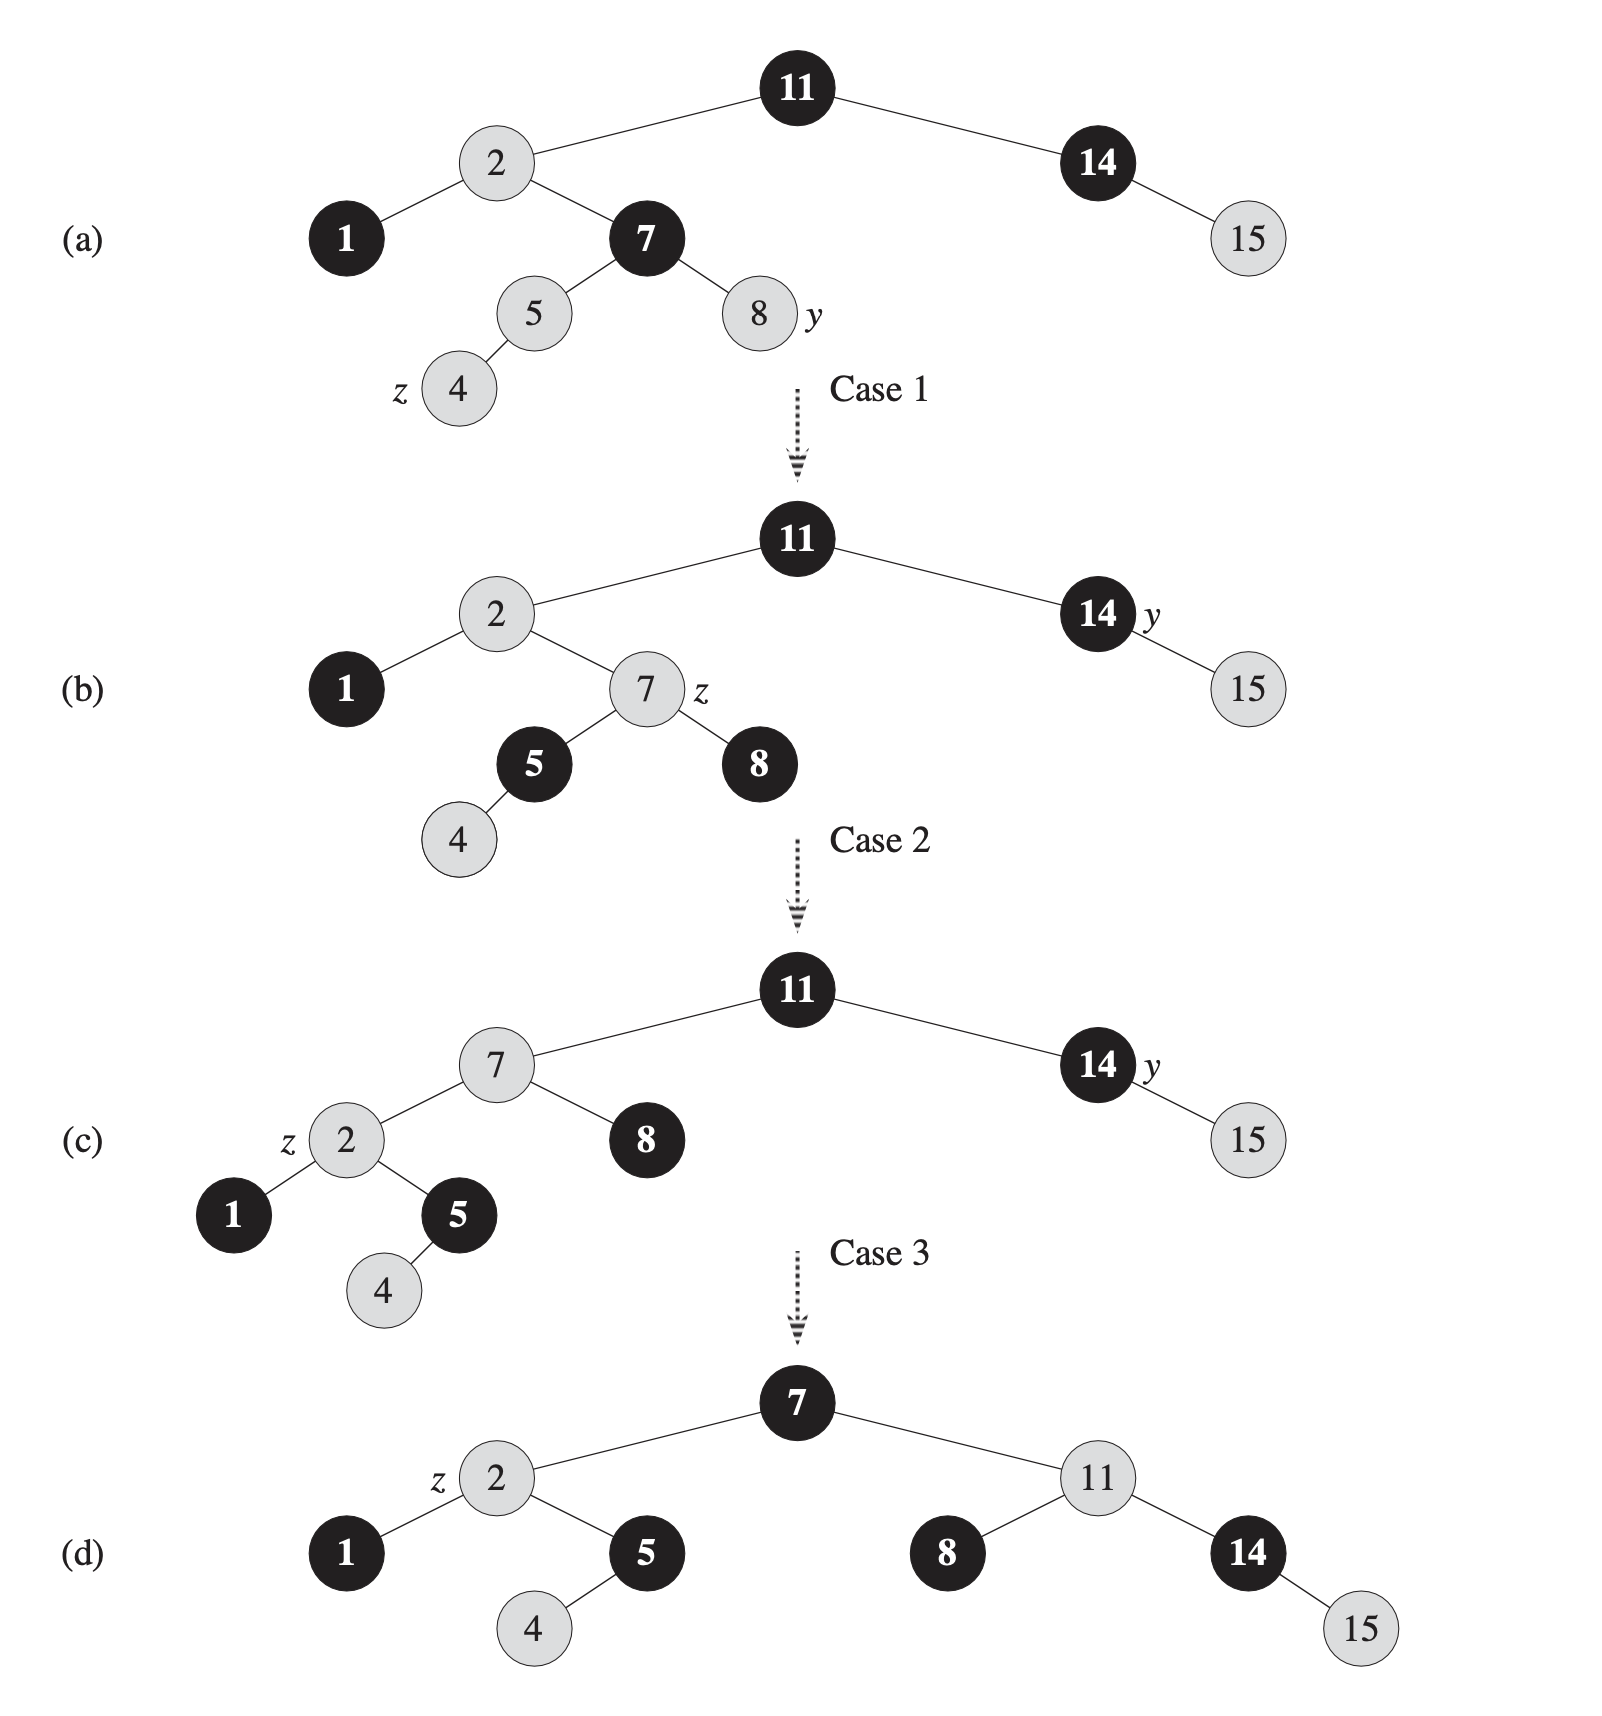
\includegraphics[width=\textwidth]{assets/insertion_rbt.png}
    \captionof{figure}{Insertion in a Red-Black Tree}
\end{minipage}

\subsubsection*{Explanation of RB-INSERT-FIXUP Algorithm}

The \texttt{RB-INSERT-FIXUP} algorithm is essential for maintaining the red-black tree properties after an insertion. Here is a step-by-step explanation of why it is necessary:

\begin{enumerate}
    \item \textbf{Initial Insertion}: When a new node $z$ is inserted, it is colored red. This is done to maintain property 5 (black-height property) without immediately violating it. However, this can lead to a violation of property 4 (no two red nodes can be adjacent).
    \item \textbf{Fixing Violations}: It checks for violations of the red-black properties, specifically property 4. If $z$'s parent $z.p$ is red, then there is a violation because $z$ and $z.p$ are both red.
    \item \textbf{Case Handling}: The algorithm handles violations through a series of cases:

        \begin{itemize}
            \item \textbf{Case 1}: If $z$'s uncle $y$ is red, both $z.p$ and $y$ are recolored to black, and $z.p.p$ is recolored to red. The algorithm then continues to check for violations up the tree.

            \item \textbf{Case 2}: If $z$ is a right child and $z.p$ is a left child, a left rotation is performed on $z.p$. This transforms the situation into Case 3.

            \item \textbf{Case 3}: $z.p$ is recolored to black, $z.p.p$ is recolored to red, and a right rotation is performed on $z.p.p$.
        \end{itemize}

        \item \textbf{Termination}: The algorithm terminates when the root is reached or when no violations are found. Finally, the root is colored black to ensure property 2 (the root is black).
\end{enumerate}

By performing these steps, the \texttt{RB-INSERT-FIXUP} algorithm ensures that all red-black tree properties are restored, maintaining the tree's balanced structure and guaranteeing efficient performance for subsequent operations.

\subsubsection*{Analysis}

What is the running time of RB-INSERT? Since the height of a red-black tree on n
nodes is $O(\log n)$, lines 1-16 of RB-INSERT take $O(\log n)$ time. In RB-INSERT-
FIXUP, the while loop repeats only if case 1 occurs, and then the pointer ´ moves
two levels up the tree. The total number of times the while loop can be executed
is therefore $O(\log n)$. Thus, RB-INSERT takes a total of $O(\log n)$ time.

\begin{observationblock}[Stopping condition]
It stops when there is one element in the array, where $p=r$.
\end{observationblock}








